\documentclass[a4paper, 10pt]{article}

\usepackage{cite}
\usepackage{color}
	\definecolor{gray}{rgb}{0.5,0.5,0.5}
\usepackage{fancyvrb}
\usepackage{graphicx}
\graphicspath{{images/}}
\DeclareGraphicsExtensions{.pdf,.png}
\usepackage{hyperref}
\usepackage{latexsym}
\usepackage{listings}
	\lstset{
		frame=single,
		numbers=left,
		numberstyle=\small\color{gray},
		tabsize=4,
	}
\usepackage{multirow}
\usepackage{setspace}
\usepackage{url}

\hyphenation{op-tical net-works semi-conduc-tor}

\def \todo#1{\textcolor{blue}{#1}}

\title{A lock-less shared memory barrier without atomic operations}
\author{Ronny Brendel\\Tutors: Sascha Kl\"uppelholz, Marcus V\"olp}

\begin{document}
\maketitle

\begin{abstract}
Today's concurrent code wastes time, because it oftentimes works in a needlessly deterministic fashion. In this report I present an extension of Mc Guire's lock-less, chaotic barrier protocol. I prove its correctness by means of checking appropriate properties on a markov decision process model. Furthermore the results of a quantitative analysis on a continuous-time markov chain model of the protocol will be evaluated. I present an implementation and evaluate its performance in comparison to two current barrier implementations. To conclude the report I repeat the main points and achievements of the work and give a perspective on possible next steps.
\end{abstract}

%%%%%%%%%%%%%%%%%%%%%%%%%%%%%%%%%%%%%%%%%%%%%%%%%%%%%%%%%%%%%%%%%%%%%%%%%%%%%%%
\section{Introduction}
Inspired by the idea of pW/CS\cite{pwcs} we intend to evaluate which other parallel synchronisation operations can be improved through stochastic algorithms. One of these operations is the barrier.

A barrier is a synchronisation primitive where all processes in a team wait until all of them reach this barrier. Torsten H\"ofler's diploma thesis\cite{hoefler2005} gives a good overview and analysis of current barrier protocols.

The barrier is a common synchronisation operation. In OpenMP\cite{omp}, by default many, operations such as for-loops, sections, and single directives invoke an implicit barrier at the end of the operation. Many distributed computing algorithms use a \emph{lock-step} approach to interleave computation with communication phases. For example a program simulating weather divides the region in question into a grid. In each of the squares on this grid the weather progression of the next 20 seconds is simulated concurrently. As a next step the squares need to exchange information such as the temperature and humidity at the borders to the neighbouring squares in order to be able to simulate the next 20 seconds. To facilitate this behaviour, barriers are used to make sure all squares finished simulating and ready to exchange data, before repeating this process.

According to a survey conducted at the HLRS\cite{rab00} the barrier is the 5th most time-consuming Message Passing Interface\cite{mpi} (MPI) operation. On average 6\% of the whole CPU time spent in MPI calls and 0.81\% of the whole program time is spent in barriers. A very small fraction of this is the actual time spent synchronizing. The majority is due to waiting for other processes to arrive, because the computation between processes is unbalanced (some take longer, some are quicker). It is still useful to pursue improvements in the barrier protocol for benchmarks and programs that require lots of synchronisation.

The report is structured as follows: First, I present the new protocol. In Section~\ref{sec:correctness} I prove its correctness. The next step is to analyse quantitative properties of the protocol. Furthermore an implementation will be evaluated and compared to the barrier implementations of GNU OpenMP\cite{gomp} and PThreads\cite{glibc}.

%%%%%%%%%%%%%%%%%%%%%%%%%%%%%%%%%%%%%%%%%%%%%%%%%%%%%%%%%%%%%%%%%%%%%%%%%%%%%%%
\section{The new protocol}
The protocol depicted in Figure~\ref{fig:barrier-source-code} went through multiple iterations, therefore it is not immediately obvious why there are two distinct loops, that look roughly the same, and what the purpose of the variable \emph{left} is.
\begin{figure}[htbp]
	\centering
	\begin{lstlisting}
shared: entry:=0, exit:=0, left:=false
local: copy, me:=2<<threadIndex, full:=(2<<numThreads)-1

if left = false {

	do {
		copy := entry
		if copy&me = 0 {
			copy |= me
			entry := copy
		}
	} while copy != full && left = false

	left := true
	exit := 0

} else if left = true {

	do {
		copy := exit
		if copy&me = 0 {
			copy |= me
			exit := copy
		}
	} while copy != full && left = true

	left := false
	entry := 0

}
	\end{lstlisting}
	\caption{Pseudo code of the barrier protocol}
	\label{fig:barrier-source-code}
\end{figure}
But let's start with an explanation on how the protocol works before going into these details.

\emph{entry} is a bitset where each bit stands for one thread having arrived in the first loop. \emph{exit} has the same role for the second loop. \emph{copy} is a local copy of entry or exit depending on the loop the thread is currently in. \emph{left} is true if one thread has left the first loop, or in other words the first barrier is completed and everyone can now leave it. Conversely if left is false, the second barrier has been completed. \emph{me} is the bit of the current thread; It is always a power of two. \emph{full} is a constant meaning all threads have successfully committed themselves to entry/exit.

Initially entry and exit are zero and left is false. A process arriving in the first loop takes a copy of entry and checks whether he is in it (\texttt{copy\&me = 0}). If not, he adds himself and writes the result back to entry. Next he checks whether everyone has committed his bit to the entry variable (\texttt{entry = full}) or at least one thread has left the loop (\texttt{left = true}). If so, he can leave and if not, he has to repeat from the point where he takes a copy of entry.

Suppose one thread has passed the first loop. He then sets left to true signalling the other threads that the barrier has been completed. All other threads will exit the loop soon, too.

Suppose one thread encounters the barrier again. Because left has been set to true after having left the previous barrier, the outermost \texttt{if} now directs the thread to the second loop and repeats the procedure described above. Instead of entry he will now use the variable exit instead. When this barrier is completed, left will be set to false, thus the third encounter will use the first loop again. Repeat. The first barrier is used on every even number of visits, and the second on every odd number of visits.

Intuitively each thread runs busily in his loop and tries to commit himself to the barrier. Since modification of the barrier variable (read until write) is not atomic, the threads rapidly overwrite each others commitment attempts. But eventually all threads will be added to entry/exit. Then the first thread, realizing that this is the case, leaves the barrier and signals all others that the barrier has been successfully completed and they can leave, too. The idea is that even though the threads read and write wildly, this approach is potentially faster than lock-based and lock-less barriers using atomic operations.

As mentioned at the start of this section, it is not obvious why left is needed. If we remove left, a race would occur where a thread leaves the first barrier and another rewrites entry to a value where the thread which has already left is not present. This thread now has no means of committing himself to entry again. Thus all threads except this one are locked inside the first loop. A deadlock occurs.

If we omit the distinction between the entry and exit loop, a thread would not be able to safely reenter the barrier while other threads are still in it. He could immediately exit it again, which is not a desired behaviour. A means of stopping this thread until all other threads have left would be necessary. Since 1 bit per process is not much memory and we can nicely distinguish between loop 1 and 2, using the variable left, this approach has been chosen.

An important assumption is that the write/read of entry and exit happen in one step. If writing to and reading from entry would take multiple steps, a deadlock scenario could be created. Thus on current computer systems this approach is limited to 32 threads. Interestingly, even on pure 64-bit systems the limit is 32. Circumventing this restriction is part of future work.

%%%%%%%%%%%%%%%%%%%%%%%%%%%%%%%%%%%%%%%%%%%%%%%%%%%%%%%%%%%%%%%%%%%%%%%%%%%%%%%
\section{Correctness of the protocol}
\label{sec:correctness}
Correctness for this protocol means it terminates and a thread can only leave the barrier if all others are present. To verify these two properties we use a markov decision process model of the protocol (Figure~\ref{fig:mdp}). To prove termination we check whether location 17 can be reached infinitely often. This implies that the protocol is deadlock-free. Two models, one in Spin\cite{spin} and one PRISM\cite{prism}, have been implemented. Both show that the protocol terminates under the mild assumption of weak fairness for scheduling threads. To prove the second part we query the model checkers whether it is possible that two threads are in different loops at the same time. Both, PRISM and Spin, show that this is not the case.

Note that in a real implementation, for example in the C programming language, it would be up to the compiler to decide in which order to evaluate the two subexpressions in the while condition. This freedom of choice is reflected in the model using non-determinism.

Intuitively the protocol terminates, because every time all processes have looped at least once, a minimum of one process has been successfully committed to the entry variable. Thus, after n repetitions, where n is the number of threads, all the processes have been registered and the barrier is completed.

\begin{figure}[htbp]
	\centering
	\includegraphics[width=4.0in]{mdp}
	\caption{Markov decision process model of the protocol}
	\label{fig:mdp}
\end{figure}

\clearpage

%%%%%%%%%%%%%%%%%%%%%%%%%%%%%%%%%%%%%%%%%%%%%%%%%%%%%%%%%%%%%%%%%%%%%%%%%%%%%%%
\section{Continuous-time markov chain for the barrier protocol}
In order to analyse quantitative properties of the protocol, we need to determine the expensive operations. Since the protocol uses shared variables to communicate, reads and writes from and to those variables are potentially costly. Each time a shared variable is modified or read, depending on the state of the cache line it is on, the operation takes a very different amount of CPU time. Therefore we consider it worthwhile to model the cache behaviour aside from the protocol itself. The cache model will be discussed in the next section. Details that are not important for the timing of the protocol, like the non-determinism in the while condition, have been omitted. The resulting CTMC is shown in Figure~\ref{fig:ctmc}. The rate of a transition is given in parenthesis.
\begin{figure}[htbp]
	\centering
	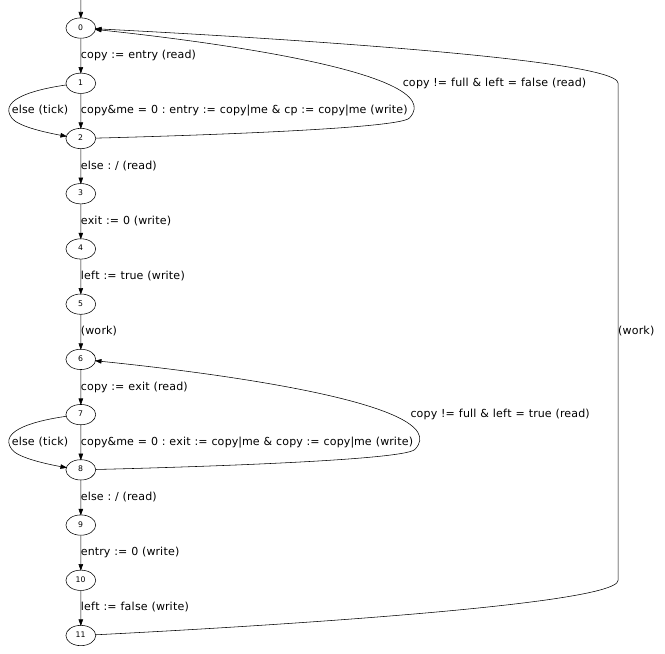
\includegraphics[width=5.2in]{ctmc}
	\caption{Continuous-time Markov chain model of the protocol}
	\label{fig:ctmc}
\end{figure}
%\clearpage
\subsection{Modeling cache behaviour}
The following description shows a very simple view on the CPU cache and omits many details of current cache protocols. This is necessary to keep the model at a manageable size.

Each CPU core has its own local copy of a cache line. A cache line copy has three distinct states. It can be \emph{modified}, which means the core has the only up-to-date copy of the cache line and all other copies are marked \emph{invalid}. It might be \emph{shared}, which means the core has an up-to-date copy, but one or more other cores have a correct copy, too. Or the cache line copy is \emph{invalid}, meaning the local copy is not up-to-date. Figure~\ref{fig:cache} shows how a cache line copy changes its state depending on events occurring. The dotted transitions are triggered by events (read/write) occurring on other cores, whereas the solid transitions are due to events issued by the own core.
\begin{figure}[htbp]
	\centering
	\includegraphics[width=2.7in]{cache}
	\caption{Model of the cache behaviour}
	\label{fig:cache}
\end{figure}

For example if a core reads a variable, it first needs to make sure that all other cores take notice and change its cache line copy state to shared in case it was modified before. After this the core fetches the cache line, marks it shared and continues reading the variable.

The timings of read and write are as follows. A read on a modified or shared variable does not imply any extra work but using the cached data. Therefore we consider this operation instantaneous. If a read is done on an invalid copy, it has to first fetch an up-to-date copy of the cache line and make sure all other cores are notified, until it can proceed. Therefore this operation takes usually around 50 CPU cycles. A write on a modified variable is instantaneous, since all other cores do not have an up-to-date copy and therefore do not have to be notified. If the cache line in question is in a shared or invalid state, we first have to wait until all other cores follow the request to invalidate their copies of the  cache line. After this we can safely write to our local copy and mark it modified. This operation usually takes around 100 cycles.

The number of cycles those operations need is strongly dependent on the CPU itself. For the model we assume a cache read to use 50 cycles and a cache write to use 100 cycles.
\subsection{Properties}
We are interested to predict how long the barrier operation takes to complete. Therefore the following three property have been chosen.
\begin{enumerate}
	\item How long does it take for one thread to pass the barrier?
	\item How long does it take for all threads to pass the barrier?
	\item If one thread has left the barrier, how long does it take until all of them complete the barrier?
\end{enumerate}

To formalise the above properties we use a continuous stochastic logic\cite{assb96}\cite{bkh99} representation. For the third query we use the \emph{conditional long-run probability}, which is explained in detail in \cite{fmix}. $n$ represents the number of threads and $t$ is a constant for the time waited in the bounded eventually ($\Diamond_{\le t} \phi$)
\begin{enumerate}
	\item $P_{=?} \big[\Diamond_{\le t} \bigvee_{1 \le i \le n} loc_i \ge 5\big]$
	\item $P_{=?} \big[\Diamond_{\le t} \bigwedge_{1 \le i \le n} loc_i \ge 5\big]$
	\item $CrlP_{=?} \big[\Diamond_{\le t} \bigwedge_{1 \le i \le n} loc_i \ge 5, \bigvee_{1 \le i \le n} (loc_i \ge 5 \wedge \bigwedge_{1 \le j \le n, i \neq j} loc_j < 5)\big]$
\end{enumerate}
\subsection{Evaluation}
The results of the queries for a barrier operation between three threads are shown in Figure~\ref{fig:one-and-all} and \ref{fig:one2all}. We can see that 90\% of the time the barrier is completed, i.e. all threads are past it, within 1000 CPU cycles. If one thread is past the barrier, all other threads will get past it in less than 380 cycles with a probability of 90\%.
\begin{figure}[htbp]
	\centering
	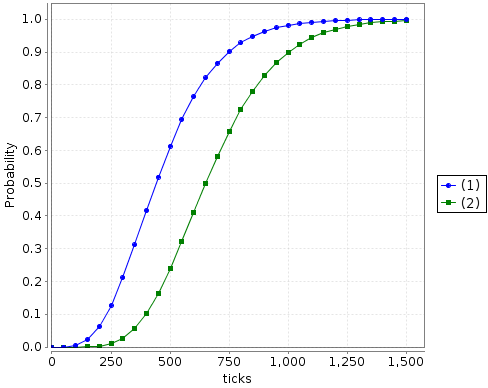
\includegraphics[width=3in]{one-and-all}
	\caption{Model checking results of query 1 and 2}
	\label{fig:one-and-all}
\end{figure}
\begin{figure}[htbp]
	\centering
	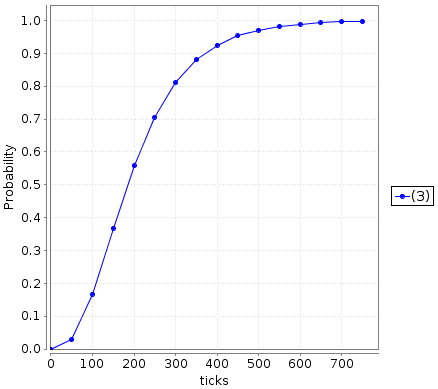
\includegraphics[width=3in]{one2all}
	\caption{Results of query 3}
	\label{fig:one2all}
\end{figure}

Note that for these queries the duration of the work period has little influence and is set to 1 cycle.

I was unable to scale this model beyond three threads, due to the huge size of the resulting state space. Future work includes tackling this limitation.

\clearpage

%%%%%%%%%%%%%%%%%%%%%%%%%%%%%%%%%%%%%%%%%%%%%%%%%%%%%%%%%%%%%%%%%%%%%%%%%%%%%%%
\section{Implementation and measurement}
\subsection{Considerations}
In order to evaluate the performance of the barrier, we spawn a certain amount of threads, repeatedly visit the barrier with a fixed number of repetitions, and afterwards end all threads. We measure the whole running time of the program. To get more reliable results we make sure the operating system's scheduler cannot reposition threads between cores, i.e., we create a one-to-one mapping between threads and cores and pin this configuration for the duration of the measurement. The implementation of the algorithm is an exact translation of the pseudocode in Figure~\ref{fig:barrier-source-code} into the C programming language.

The measurements were conducted on a 64 thread, 32 core and 4 socket AMD Opteron\texttrademark 6274 system.
\subsection{Evaluation}
The results are shown in Figure~\ref{fig:measurement-1} and \ref{fig:measurement-2}. Due to time constraints, the measurements are not 100 percent reliable. They should give an intuition in which ballpark the performance is, though.
\begin{figure}[htbp]
	\centering
	\begin{tabular}{r | l l l }
		threads & OpenMP  & PThreads  & new \\
		\hline
		 4      & 3.3s    & 3.5s      & 0.2s \\
		 8      & 3.3s    & 3.5s      & 0.3s \\
		16      & 3.2s    & 3.7s      & 0.6s \\
		32      & 5.0s    & 5.5s      & 1.4s \\
	\end{tabular}
	\caption{Measurement results for consecutive barrier visits without delay}
	\label{fig:measurement-1}
\end{figure}

When not having any delay, but rather repeating the barrier as quickly as possible, the new protocol outperforms GNU OpenMP's and libc's pthreads implementation by far. This is likely due to the fact that both of them are lock-based and spend considerable time waiting for callbacks.

\begin{figure}[htbp]
	\centering
	\begin{tabular}{r | l l l}
		threads & OpenMP & PThreads & new \\
		\hline
		 4      & 5.1s   & 5.1s     & 4.6s \\
		 8      & 5.5s   & 5.5s     & 4.8s \\
		16      & 5.9s   & 5.9s     & 5.1s \\
		32      & 7.0s   & 7.0s     & 6.1s \\
	\end{tabular}
	\caption{Measurement results for barrier visits with 1ms delay}
	\label{fig:measurement-2}
\end{figure}

When adding one millisecond (roughly two million cycles) of waiting time, the runtime of the new barrier still finishes roughly 10\% earlier.

A minor drawback of the new barrier protocol is that the intended false-sharing of the cache line, with the variables on it, adds strain to the cache bandwidth. Measurements show that about 1\% of the total cache bandwidth is lost, regardless of the thread count. The percentage is this low, because the speed of false-sharing is limited by the waiting time for transferring a cache line between two caches and the time it takes to invalidate the line on all other caches.

Another drawback is that due to the busy waiting, the total number CPU cycles used by the protocol is way larger than for callback-based approaches. In a setting were performance is important this would not be a problem, because the CPU does not spend the cycles saved on any 'real work'. But it would indeed save energy to remove strain from the CPU.

There exist approaches to reduce the negative effects of both these problems. This will be part of future work.

%%%%%%%%%%%%%%%%%%%%%%%%%%%%%%%%%%%%%%%%%%%%%%%%%%%%%%%%%%%%%%%%%%%%%%%%%%%%%%%
\section{Conclusion}
In this report I presented a new barrier protocol, whose main difference to existing protocols is, that it neither relies on locking mechanisms nor atomic operations.
In its current state the number of threads supported by this protocol is limited to the number of bits a read/write can transfer in one uninterceptable operation -- 32 on current generation CPUs.
I proved the correctness of the protocol by checking an MDP model in two different model checkers for potential deadlocks and inconsistencies.
Furthermore I presented a brief analysis of a CTMC model showing some basic properties of the protocol.
Moreover we saw that a straight forward implementation of the new barrier is significantly faster than two currently used barrier implementations.

%%%%%%%%%%%%%%%%%%%%%%%%%%%%%%%%%%%%%%%%%%%%%%%%%%%%%%%%%%%%%%%%%%%%%%%%%%%%%%%
\section{Future Work}
Due to time-constraints, much of what needs to be done is enumerated in this section.

The CTMC model of the protocol is already too large to be analysed when being used with four threads. One should explore ways to reduce its size. Common approaches include symmetry reduction, partial order reduction and reducing the model manually depending on the properties to be checked. Once this has been achieved, further quantitative analysis on the model seems worthwhile.

There are various possibilities to make an actual implementation faster and/or more resource-friendly than the straight forward one shown in this report. For example one could experiment with using the \emph{mwait} instruction in order to wait for changes in a shared variable, thus not having to actively poll it. Another way to speed up the protocol is that a thread keeps track of which other threads he has already seen inside the barrier and does not only commit himself to the it but the other threads he has seen, too.

One should also explore ways to circumvent the current 32 thread limit.

Another interesting pursuit is to evaluate ways to modify the protocol in order to make it work in a distributed setting, thus making it an alternative to current distributed memory barrier protocols.

%%%%%%%%%%%%%%%%%%%%%%%%%%%%%%%%%%%%%%%%%%%%%%%%%%%%%%%%%%%%%%%%%%%%%%%%%%%%%%%
\nocite{*} % give out non cited references
\bibliographystyle{abbrv}
\bibliography{references}{}

\end{document}
